% Generated by scripts/build_latex.py from docs/report/ch7_results.md: edit the Markdown, not this file.
\chapter{Results and Discussion}\label{ch:7}

All numbers in this chapter come from the offline evaluation script \code{scripts/\allowbreak{}evaluate.\allowbreak{}py} (full output in \code{docs/\allowbreak{}results/\allowbreak{}evaluation.\allowbreak{}md} and \code{evaluation.json}) and from the Step 4 / Step 5 benchmark (\code{docs/\allowbreak{}results/\allowbreak{}step4\_\allowbreak{}benchmark.\allowbreak{}md}).

\FloatBarrier
\section{Experimental Setup}\label{sec:7.1}

\textbf{Datasets.} We generated five datasets ourselves with \code{scripts/\allowbreak{}make\_\allowbreak{}samples.\allowbreak{}py} from fixed random seeds (Table~\ref{tab:7.1}). \textbf{All five are synthetic}: they describe no real people or companies and their generating processes are known. They were designed to be realistic in shape --- missing values, categorical columns, class imbalance, seasonality, overlapping clusters --- and to cover the four task families.

\begin{table}[H]
\centering
\linespread{1}\footnotesize
\setlength{\tabcolsep}{4pt}
\caption{Evaluation datasets (synthetic, seeded)}\label{tab:7.1}
\begin{tabular}{|>{\raggedright\arraybackslash\hspace{0pt}}p{\dimexpr 0.1216\linewidth-2\tabcolsep-2\arrayrulewidth\relax}|>{\raggedright\arraybackslash\hspace{0pt}}p{\dimexpr 0.1903\linewidth-2\tabcolsep-2\arrayrulewidth\relax}|>{\raggedleft\arraybackslash\hspace{0pt}}p{\dimexpr 0.0873\linewidth-2\tabcolsep-2\arrayrulewidth\relax}|>{\raggedleft\arraybackslash\hspace{0pt}}p{\dimexpr 0.1101\linewidth-2\tabcolsep-2\arrayrulewidth\relax}|>{\raggedright\arraybackslash\hspace{0pt}}p{\dimexpr 0.1903\linewidth-2\tabcolsep-2\arrayrulewidth\relax}|>{\raggedright\arraybackslash\hspace{0pt}}p{\dimexpr 0.1903\linewidth-2\tabcolsep-2\arrayrulewidth\relax}|>{\raggedright\arraybackslash\hspace{0pt}}p{\dimexpr 0.1102\linewidth-2\tabcolsep-2\arrayrulewidth\relax}|}
\hline
\rowcolor{tableheader}\textbf{Dataset} & \textbf{File} & \textbf{Rows} & \textbf{Columns} & \textbf{Task} & \textbf{Target} & \textbf{Notes} \\
\hline
Churn & \code{customer\_\allowbreak{}churn.csv} & 3,000 & 12 & Binary classification & \code{churn} & 985 ``Yes'' (32.8\%) \\ \hline
Crop price & \code{crop\_\allowbreak{}price.csv} & 2,000 & 11 & Regression & \code{price} & 106 missing cells \\ \hline
Store sales & \code{store\_\allowbreak{}sales.csv} & 730 & 6 & Forecasting & \code{sales} & Daily, two years \\ \hline
Delivery & \code{delivery\_\allowbreak{}status.\allowbreak{}csv} & 2,500 & 12 & 3-class classification & \code{delivery\_\allowbreak{}status} & 1,375 / 750 / 375 \\ \hline
Segments & \code{customer\_\allowbreak{}segments.\allowbreak{}csv} & 1,600 & 8 & Clustering & \code{segment} (scoring only) & Four groups \\ \hline
\end{tabular}
\end{table}

\textbf{Protocol.} Three seeds (42, 43, 44); every number is the mean \ensuremath{\pm}~sample standard deviation. The seed controls the split (chronological for time series), Optuna's sampler, the models and the perturbations. The \textbf{fast} budget was used (3 models \ensuremath{\times} 15 trials, 60 s per model, 180 s total; one re-plan with the full budget after a failed verification). The real Orchestrator ran in \textbf{offline mode}: requirements came from the data profile, and Segments was given an explicit clustering requirement whose \code{segment} column is used only for scoring. Models were selected on the validation split and the test split (10\%) was read once. \textbf{Environment:} Python 3.12.0, Windows 11, 16 logical CPUs, scikit-learn 1.9.1, XGBoost 3.4.1, LightGBM 4.7.0, Optuna 5.0.0, SHAP 0.52.0. The evaluation took 1,081.5 s, plus two short Segments re-runs (Section~\ref{sec:7.7}).

\textbf{Metrics.} F1 for classification (binary F1 of the positive class; weighted F1 for Delivery), RMSE for regression and forecasting, and the adjusted Rand index (ARI) for clustering. Each model is compared with a trivial baseline on the same test split: the majority class, the mean, the seasonal naive forecast or a random cluster assignment.

\FloatBarrier
\section{Main Benchmark}\label{sec:7.2}

\begin{table}[H]
\centering
\linespread{1}\fontsize{9}{11}\selectfont
\setlength{\tabcolsep}{3pt}
\caption{Main benchmark (full system, clean data, mean \ensuremath{\pm}~std over 3 seeds)}\label{tab:7.2}
\begin{tabular}{|>{\raggedright\arraybackslash\hspace{0pt}}p{\dimexpr 0.1134\linewidth-2\tabcolsep-2\arrayrulewidth\relax}|>{\raggedright\arraybackslash\hspace{0pt}}p{\dimexpr 0.1342\linewidth-2\tabcolsep-2\arrayrulewidth\relax}|>{\raggedright\arraybackslash\hspace{0pt}}p{\dimexpr 0.0927\linewidth-2\tabcolsep-2\arrayrulewidth\relax}|>{\raggedleft\arraybackslash\hspace{0pt}}p{\dimexpr 0.0822\linewidth-2\tabcolsep-2\arrayrulewidth\relax}|>{\raggedleft\arraybackslash\hspace{0pt}}p{\dimexpr 0.1134\linewidth-2\tabcolsep-2\arrayrulewidth\relax}|>{\raggedleft\arraybackslash\hspace{0pt}}p{\dimexpr 0.1446\linewidth-2\tabcolsep-2\arrayrulewidth\relax}|>{\raggedleft\arraybackslash\hspace{0pt}}p{\dimexpr 0.0822\linewidth-2\tabcolsep-2\arrayrulewidth\relax}|>{\raggedleft\arraybackslash\hspace{0pt}}p{\dimexpr 0.1238\linewidth-2\tabcolsep-2\arrayrulewidth\relax}|>{\raggedleft\arraybackslash\hspace{0pt}}p{\dimexpr 0.1136\linewidth-2\tabcolsep-2\arrayrulewidth\relax}|}
\hline
\rowcolor{tableheader}\textbf{Dataset} & \textbf{Best model (seeds)} & \textbf{Metric} & \textbf{Test score} & \textbf{Baseline} & \textbf{Improvement} & \textbf{Train time (s)} & \textbf{Inference (ms/row)} & \textbf{Verified} \\
\hline
Churn & logistic regression (3/3) & F1 \ensuremath{\uparrow} & 0.649 \ensuremath{\pm}~0.028 & 0.000 & n/a\textsuperscript{1} & 19.8 \ensuremath{\pm}~2.5 & 0.0286 \ensuremath{\pm}~0.0045 & 3/3 \\ \hline
Crop price & LightGBM (3/3) & RMSE \ensuremath{\downarrow} & 356.9 \ensuremath{\pm}~26.81 & 2,392.8 \ensuremath{\pm}~45.77 & +85.1\% \ensuremath{\pm}~0.8 & 7.0 \ensuremath{\pm}~0.5 & 0.0610 \ensuremath{\pm}~0.0073 & 3/3 \\ \hline
Store sales & ridge (3/3) & RMSE \ensuremath{\downarrow} & 923.6 \ensuremath{\pm}~0.000 & 2,340.7 \ensuremath{\pm}~0.000 & +60.5\% \ensuremath{\pm}~0.0 & 4.3 \ensuremath{\pm}~1.1 & 0.2011 \ensuremath{\pm}~0.0148 & 3/3 \\ \hline
Delivery & logistic regression (2/3) & F1 \ensuremath{\uparrow} & 0.656 \ensuremath{\pm}~0.024 & 0.393 \ensuremath{\pm}~0.000 & +67.0\% \ensuremath{\pm}~6.1 & 72.2 \ensuremath{\pm}~74.2 & 0.0440 \ensuremath{\pm}~0.0226 & 2/3 \\ \hline
Segments & Gaussian mixture (3/3) & ARI \ensuremath{\uparrow} & 0.816 \ensuremath{\pm}~0.045 & 0.004 \ensuremath{\pm}~0.007 & n/a\textsuperscript{1} & 2.7 \ensuremath{\pm}~0.4 & 0.0159 \ensuremath{\pm}~0.0036 & 3/3 \\ \hline
\end{tabular}
\end{table}

\ensuremath{\uparrow} higher is better, \ensuremath{\downarrow} lower is better. \textit{Train time} covers the whole search plus the final refit; \textit{inference} is the median time of the fitted pipeline on up to 500 test rows. \textsuperscript{1} The baseline is at chance level (below 0.05), so a relative improvement is undefined: the majority class never predicts churn (F1 = 0) and random clusters have an ARI of about 0.

The full system \textbf{beat the baseline on all five datasets}, reducing RMSE by 85.1\% on crop price and 60.5\% on store sales. Simple models were often selected --- logistic regression on churn and delivery, ridge on store sales --- which suggests that these synthetic datasets are close to linear (Figure~\ref{fig:7.1}).

\begin{figure}[htbp]
  \centering
  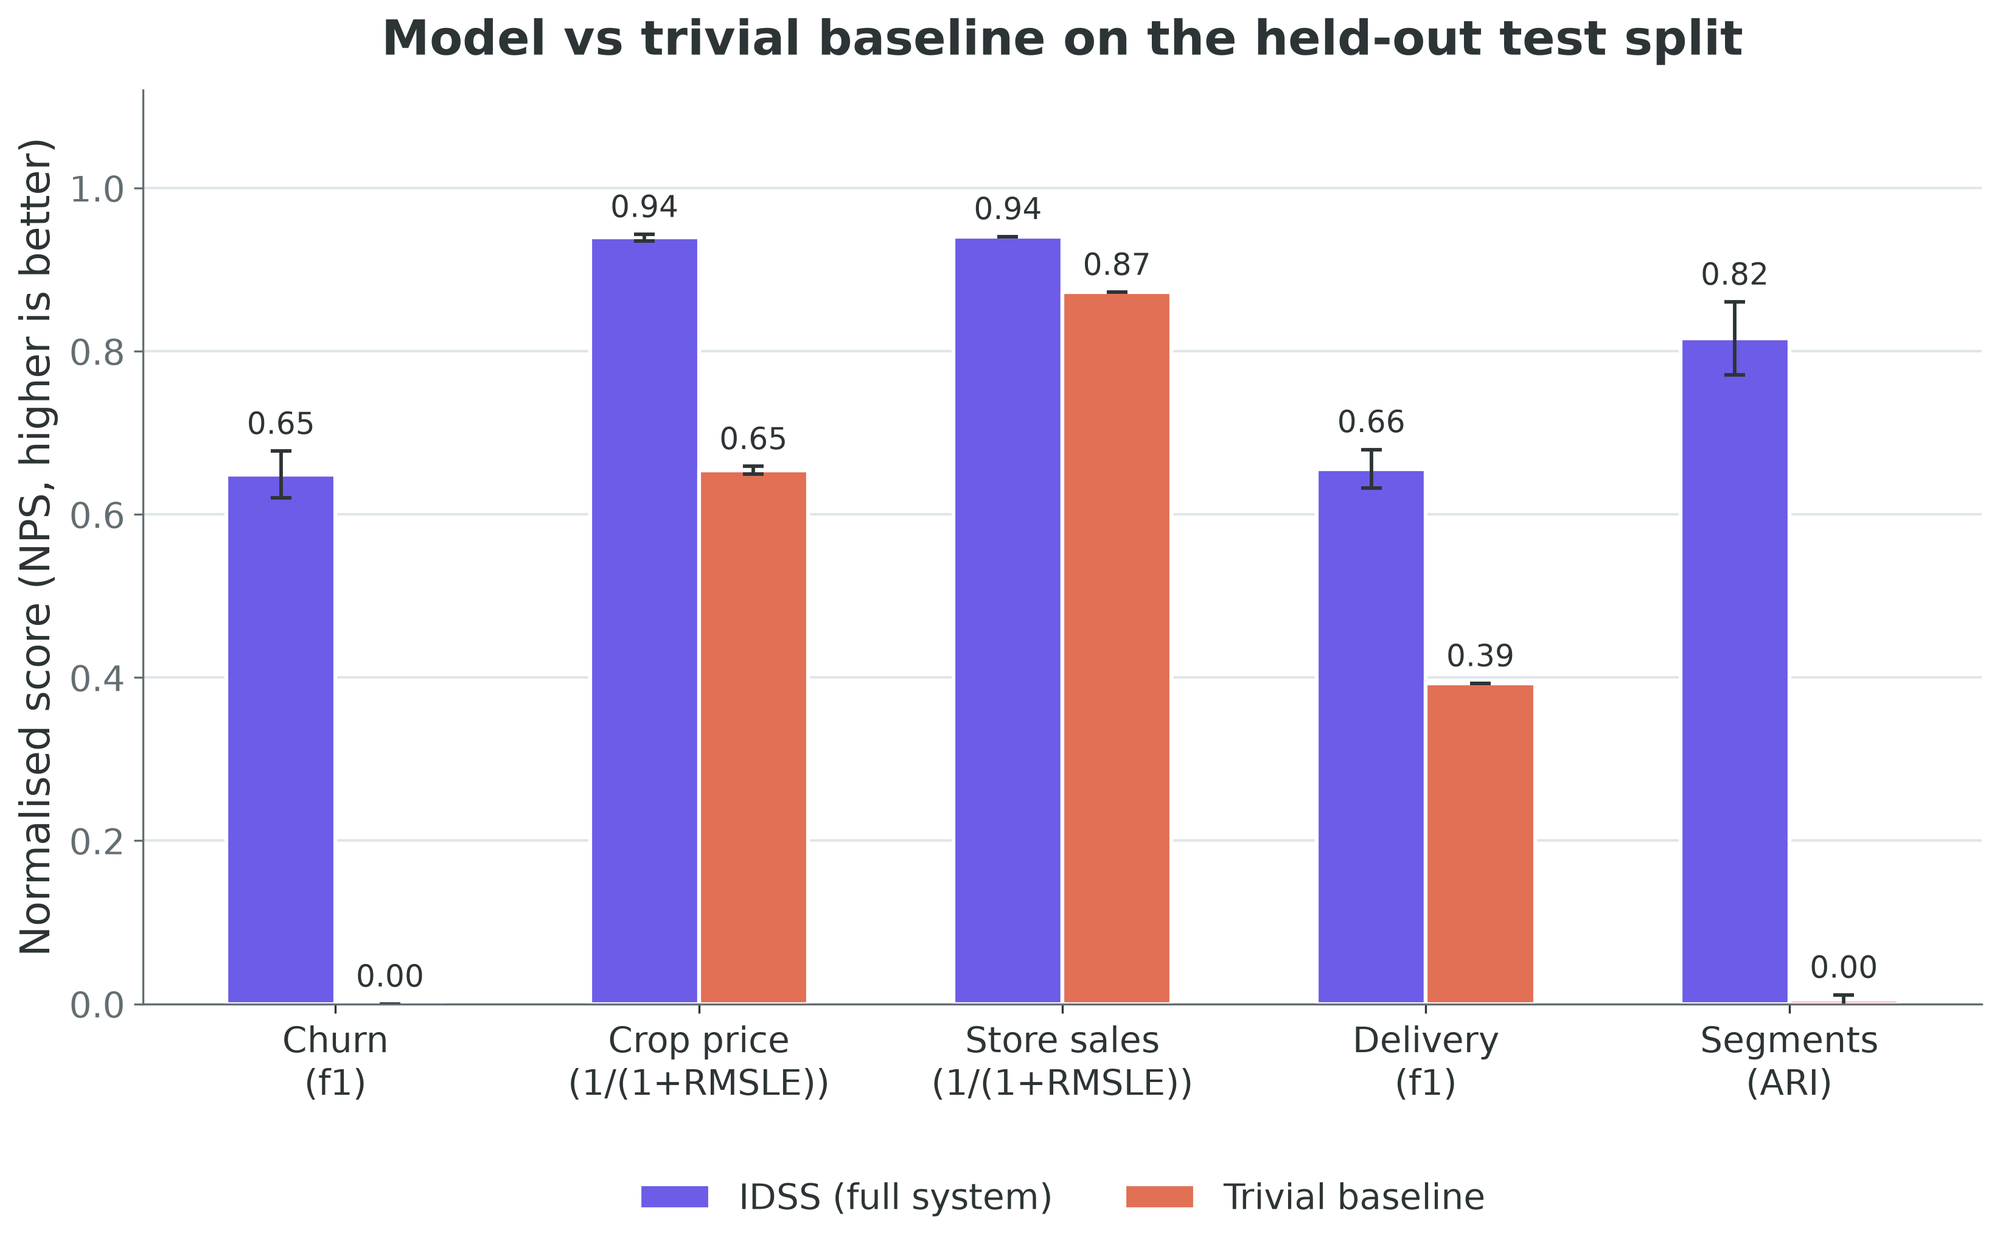
\includegraphics[width=\linewidth,height=7.3in,keepaspectratio]{figures/benchmark_vs_baseline.png}
  \caption{Model versus trivial baseline on the held-out test split (normalised score)}\label{fig:7.1}
\end{figure}

\FloatBarrier
\section{Paper-style Metrics: SR, NPS and CS}\label{sec:7.3}

Following AutoML-Agent \cite{ref9}:

\begin{quote}
\textbf{SR} = runs that complete the whole pipeline (trained, tested, verified, explained, PDF report) \ensuremath{\div} all runs; \textbf{NPS} = the test score for 0--1 metrics (F1; ARI clipped at 0), or 1 / (1 + RMSLE) for regression and forecasting, and 0 for a failed run; \textbf{CS} = 0.5 \ensuremath{\cdot} SR + 0.5 \ensuremath{\cdot} NPS.
\end{quote}

RMSLE = \ensuremath{\surd}( (1/\textit{n}) \ensuremath{\Sigma} (log(1 + \textit{\ensuremath{\hat{y}}}) \ensuremath{-} log(1 + \textit{y}))\textsuperscript{2} ) is scale-free; 1 / (1 + RMSE) would depend on the units of the target and be close to 0 for prices or daily sales. The overall value is the mean over datasets per seed, then over seeds.

\begin{table}[H]
\centering
\linespread{1}\small
\setlength{\tabcolsep}{4pt}
\caption{SR, NPS and CS (mean \ensuremath{\pm}~std over 3 seeds)}\label{tab:7.3}
\begin{tabular}{|>{\raggedright\arraybackslash\hspace{0pt}}p{\dimexpr 0.1783\linewidth-2\tabcolsep-2\arrayrulewidth\relax}|>{\raggedright\arraybackslash\hspace{0pt}}p{\dimexpr 0.2248\linewidth-2\tabcolsep-2\arrayrulewidth\relax}|>{\raggedleft\arraybackslash\hspace{0pt}}p{\dimexpr 0.1989\linewidth-2\tabcolsep-2\arrayrulewidth\relax}|>{\raggedleft\arraybackslash\hspace{0pt}}p{\dimexpr 0.1989\linewidth-2\tabcolsep-2\arrayrulewidth\relax}|>{\raggedleft\arraybackslash\hspace{0pt}}p{\dimexpr 0.1989\linewidth-2\tabcolsep-2\arrayrulewidth\relax}|}
\hline
\rowcolor{tableheader}\textbf{Dataset} & \textbf{NPS from} & \textbf{SR} & \textbf{NPS} & \textbf{CS} \\
\hline
Churn & F1 & 1.000 \ensuremath{\pm}~0.000 & 0.649 \ensuremath{\pm}~0.028 & 0.825 \ensuremath{\pm}~0.014 \\ \hline
Crop price & 1 / (1 + RMSLE) & 1.000 \ensuremath{\pm}~0.000 & 0.939 \ensuremath{\pm}~0.004 & 0.970 \ensuremath{\pm}~0.002 \\ \hline
Store sales & 1 / (1 + RMSLE) & 1.000 \ensuremath{\pm}~0.000 & 0.941 \ensuremath{\pm}~0.000 & 0.970 \ensuremath{\pm}~0.000 \\ \hline
Delivery & F1 & 1.000 \ensuremath{\pm}~0.000 & 0.656 \ensuremath{\pm}~0.024 & 0.828 \ensuremath{\pm}~0.012 \\ \hline
Segments & ARI & 1.000 \ensuremath{\pm}~0.000 & 0.816 \ensuremath{\pm}~0.045 & 0.908 \ensuremath{\pm}~0.022 \\ \hline
\textbf{Overall} &  & \textbf{1.000 \ensuremath{\pm}~0.000} & \textbf{0.800 \ensuremath{\pm}~0.011} & \textbf{0.900 \ensuremath{\pm}~0.005} \\ \hline
\end{tabular}
\end{table}

\begin{figure}[htbp]
  \centering
  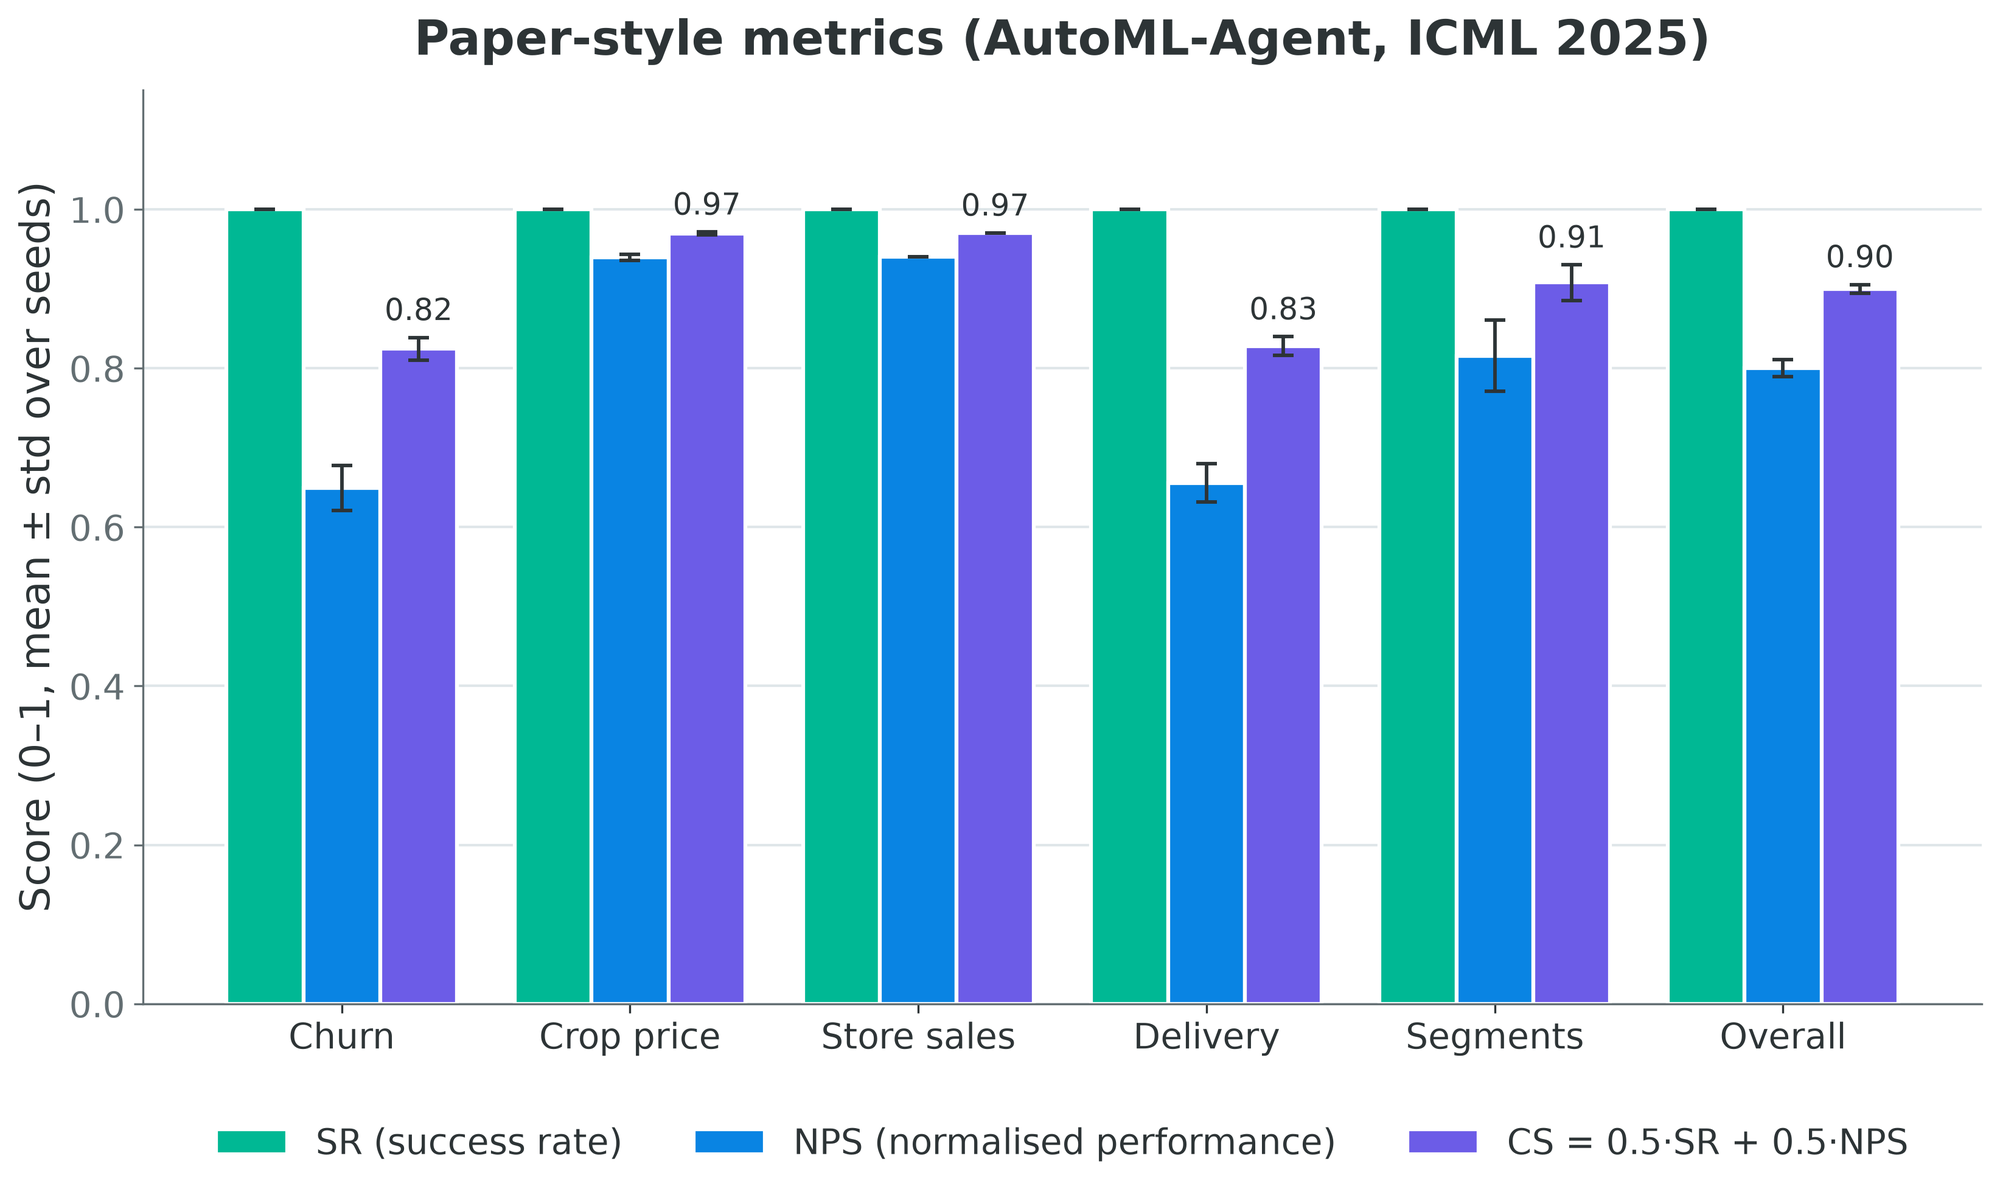
\includegraphics[width=\linewidth,height=7.3in,keepaspectratio]{figures/paper_metrics.png}
  \caption{Paper-style metrics (SR, NPS, CS) per dataset}\label{fig:7.2}
\end{figure}

All 15 runs completed end to end (SR = 1.00). Because IDSS runs tested code instead of LLM-written scripts, every run that starts also finishes, so SR measures robustness rather than code quality, and NPS carries the differences. \textbf{These numbers cannot be compared with the AutoML-Agent paper's tables}: datasets, budgets and success criteria differ.

\FloatBarrier
\section{Ablation Study}\label{sec:7.4}

One component was removed at a time: \textbf{\ensuremath{-} threshold tuning} (cut-off fixed at 0.5), \textbf{\ensuremath{-} hyperparameter tuning} (library defaults), \textbf{\ensuremath{-} verification re-planning} (first attempt is final) and a \textbf{single-model baseline} (one default LightGBM, or k-means for clustering, with none of the above). Ablation runs stop after verification. Table~\ref{tab:7.4} shows the test score and, in brackets, the change against the full system on the same seed (positive = better).

\begin{table}[H]
\centering
\linespread{1}\fontsize{9}{11}\selectfont
\setlength{\tabcolsep}{3pt}
\caption{Ablation study (mean \ensuremath{\pm}~std over 3 seeds)}\label{tab:7.4}
\begin{tabular}{|>{\raggedright\arraybackslash\hspace{0pt}}p{\dimexpr 0.1796\linewidth-2\tabcolsep-2\arrayrulewidth\relax}|>{\raggedleft\arraybackslash\hspace{0pt}}p{\dimexpr 0.1159\linewidth-2\tabcolsep-2\arrayrulewidth\relax}|>{\raggedleft\arraybackslash\hspace{0pt}}p{\dimexpr 0.1052\linewidth-2\tabcolsep-2\arrayrulewidth\relax}|>{\raggedleft\arraybackslash\hspace{0pt}}p{\dimexpr 0.1159\linewidth-2\tabcolsep-2\arrayrulewidth\relax}|>{\raggedleft\arraybackslash\hspace{0pt}}p{\dimexpr 0.1159\linewidth-2\tabcolsep-2\arrayrulewidth\relax}|>{\raggedleft\arraybackslash\hspace{0pt}}p{\dimexpr 0.1159\linewidth-2\tabcolsep-2\arrayrulewidth\relax}|>{\raggedleft\arraybackslash\hspace{0pt}}p{\dimexpr 0.0840\linewidth-2\tabcolsep-2\arrayrulewidth\relax}|>{\raggedleft\arraybackslash\hspace{0pt}}p{\dimexpr 0.0840\linewidth-2\tabcolsep-2\arrayrulewidth\relax}|>{\raggedleft\arraybackslash\hspace{0pt}}p{\dimexpr 0.0839\linewidth-2\tabcolsep-2\arrayrulewidth\relax}|}
\hline
\rowcolor{tableheader}\textbf{Variant} & \textbf{Churn (F1)} & \textbf{Crop price (RMSE)} & \textbf{Store sales (RMSE)} & \textbf{Delivery (F1)} & \textbf{Segments (ARI)} & \textbf{NPS} & \textbf{CS} & \textbf{Train time (s)} \\
\hline
\textbf{Full system} & 0.649 \ensuremath{\pm}~0.028 & 356.9 \ensuremath{\pm}~26.81 & 923.6 \ensuremath{\pm}~0.000 & 0.656 \ensuremath{\pm}~0.024 & 0.816 \ensuremath{\pm}~0.045 & 0.800 \ensuremath{\pm}~0.011 & \textbf{0.900 \ensuremath{\pm}~0.005} & 21.2 \ensuremath{\pm}~39.0 \\ \hline
\ensuremath{-} threshold tuning & 0.561 \ensuremath{\pm}~0.006 (\ensuremath{-}13.4\%) & same\textsuperscript{2} & same\textsuperscript{2} & same\textsuperscript{2} & same\textsuperscript{2} & 0.782 \ensuremath{\pm}~0.005 & 0.891 \ensuremath{\pm}~0.003 & 26.3 \ensuremath{\pm}~43.5 \\ \hline
\ensuremath{-} hyperparameter tuning & 0.648 \ensuremath{\pm}~0.027 (\ensuremath{-}0.1\%) & 378.5 \ensuremath{\pm}~52.63 (\ensuremath{-}5.7\%) & 915.7 \ensuremath{\pm}~0.000 (+0.9\%) & 0.669 \ensuremath{\pm}~0.021 (+2.0\%) & 0.523 \ensuremath{\pm}~0.078 (\ensuremath{-}35.6\%) & 0.743 \ensuremath{\pm}~0.018 & 0.871 \ensuremath{\pm}~0.009 & 1.9 \ensuremath{\pm}~1.5 \\ \hline
\ensuremath{-} verification re-planning & 0.649 \ensuremath{\pm}~0.028 (+0.0\%) & 356.9 \ensuremath{\pm}~26.81 (+0.0\%) & 923.6 \ensuremath{\pm}~0.000 (+0.0\%) & 0.656 \ensuremath{\pm}~0.024 (+0.0\%) & 0.816 \ensuremath{\pm}~0.045 (+0.0\%) & 0.800 \ensuremath{\pm}~0.011 & 0.900 \ensuremath{\pm}~0.005 & 12.8 \ensuremath{\pm}~11.0 \\ \hline
Single-model baseline & 0.521 \ensuremath{\pm}~0.057 (\ensuremath{-}19.3\%) & 368.4 \ensuremath{\pm}~41.67 (\ensuremath{-}3.0\%) & 1,298.8 \ensuremath{\pm}~0.000 (\ensuremath{-}40.6\%) & 0.648 \ensuremath{\pm}~0.020 (\ensuremath{-}1.1\%) & 0.508 \ensuremath{\pm}~0.012 (\ensuremath{-}37.6\%) & 0.707 \ensuremath{\pm}~0.016 & 0.854 \ensuremath{\pm}~0.008 & 0.7 \ensuremath{\pm}~0.4 \\ \hline
\end{tabular}
\end{table}

SR was 1.000 for every variant. \textsuperscript{2} Threshold tuning applies only to binary classification; the other datasets reuse the full-system runs.

\begin{figure}[htbp]
  \centering
  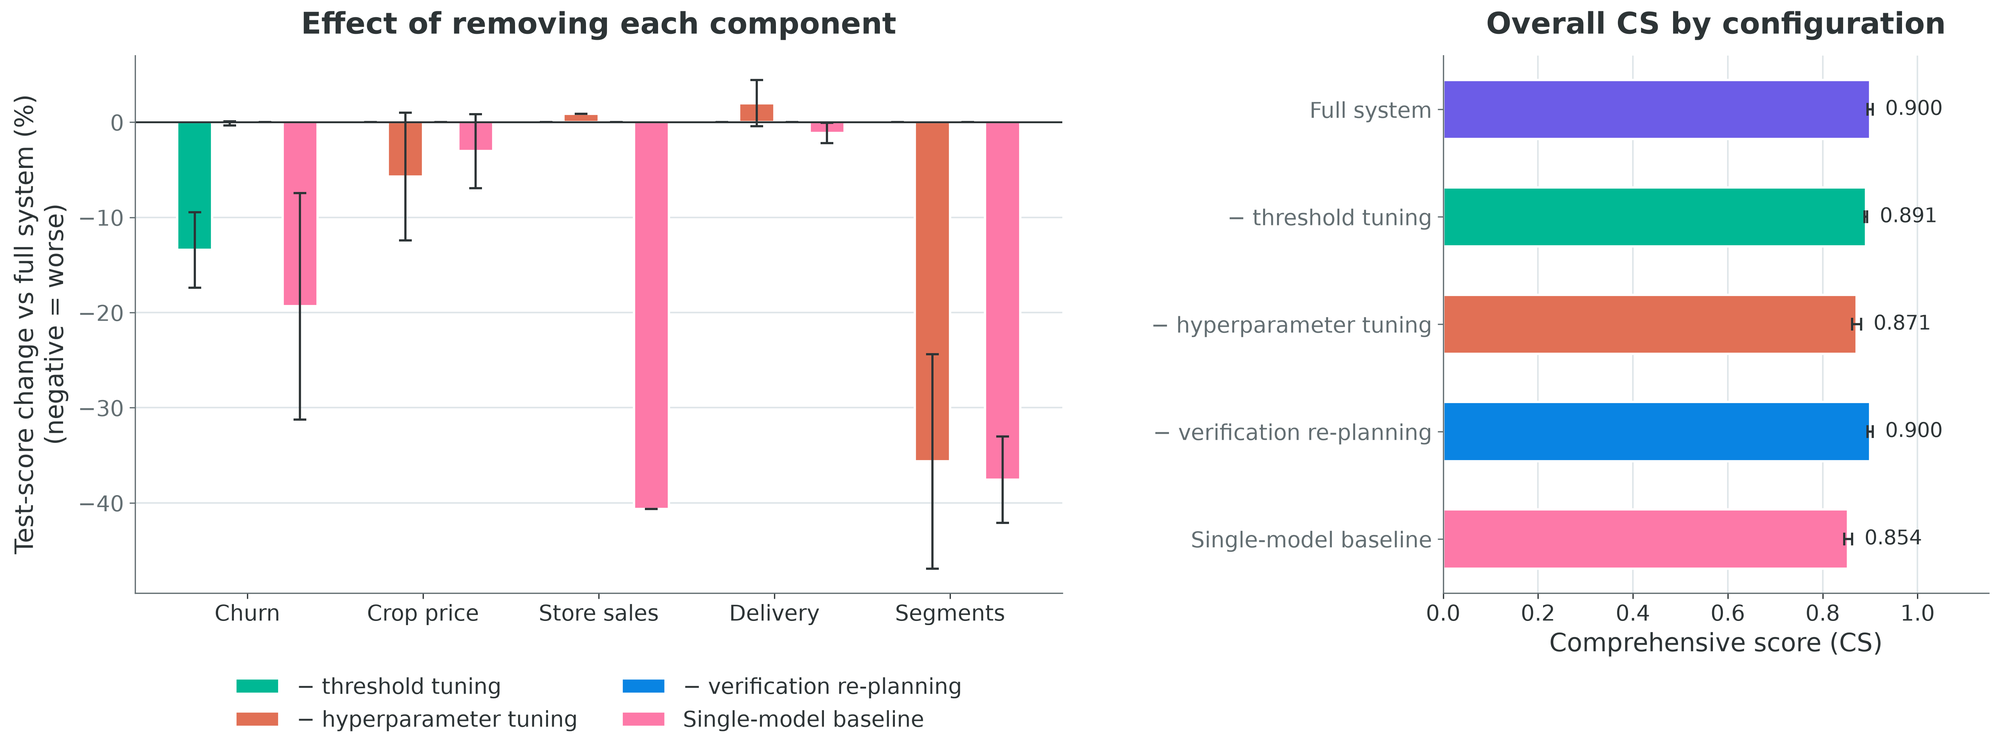
\includegraphics[width=\linewidth,height=7.3in,keepaspectratio]{figures/ablation.png}
  \caption{Ablation study: change of the test score per component and overall CS}\label{fig:7.3}
\end{figure}

\begin{itemize}
  \item \textbf{Threshold tuning} matters only for binary classification, but there it matters a lot: \ensuremath{-}13.4\% F1 on churn without it (Section~\ref{sec:7.6}).
  \item \textbf{Hyperparameter tuning} raises CS from 0.871 to 0.900. Without it, Segments loses 35.6\% (tuning finds the right number of clusters), while Delivery gains 2.0\%; where defaults scored higher on the test split, tuning had still chosen the best model on the validation split, a difference within selection noise on near-linear data.
  \item \textbf{Verification re-planning} was triggered in 1 of 15 clean full-system runs and did not change the score. Across all configurations it ran three times and the second attempt never passed; the system then reports \textit{not verified} (Section~\ref{sec:7.9}).
  \item \textbf{The single default model} reaches CS = 0.854 against 0.900 and passes verification in only 6 of 15 runs (full system: 14 of 15), with the largest losses on store sales (\ensuremath{-}40.6\%), segments (\ensuremath{-}37.6\%) and churn (\ensuremath{-}19.3\%).
\end{itemize}

\FloatBarrier
\section{Robustness}\label{sec:7.5}

The full system was re-run on corrupted copies of each dataset: \textbf{+10\% missing values} (cells blanked at random in all columns except the target, identifiers and the time index) and \textbf{+5 noisy columns} (three numeric, one integer, one categorical).

\begin{table}[H]
\centering
\linespread{1}\footnotesize
\setlength{\tabcolsep}{4pt}
\caption{Robustness (mean \ensuremath{\pm}~std over 3 seeds; change vs clean data, negative = worse)}\label{tab:7.5}
\begin{tabular}{|>{\raggedright\arraybackslash\hspace{0pt}}p{\dimexpr 0.1359\linewidth-2\tabcolsep-2\arrayrulewidth\relax}|>{\raggedright\arraybackslash\hspace{0pt}}p{\dimexpr 0.1067\linewidth-2\tabcolsep-2\arrayrulewidth\relax}|>{\raggedleft\arraybackslash\hspace{0pt}}p{\dimexpr 0.1059\linewidth-2\tabcolsep-2\arrayrulewidth\relax}|>{\raggedleft\arraybackslash\hspace{0pt}}p{\dimexpr 0.1307\linewidth-2\tabcolsep-2\arrayrulewidth\relax}|>{\raggedleft\arraybackslash\hspace{0pt}}p{\dimexpr 0.1169\linewidth-2\tabcolsep-2\arrayrulewidth\relax}|>{\raggedleft\arraybackslash\hspace{0pt}}p{\dimexpr 0.1322\linewidth-2\tabcolsep-2\arrayrulewidth\relax}|>{\raggedleft\arraybackslash\hspace{0pt}}p{\dimexpr 0.1139\linewidth-2\tabcolsep-2\arrayrulewidth\relax}|>{\raggedleft\arraybackslash\hspace{0pt}}p{\dimexpr 0.1577\linewidth-2\tabcolsep-2\arrayrulewidth\relax}|}
\hline
\rowcolor{tableheader}\textbf{Dataset} & \textbf{Metric} & \textbf{Clean} & \textbf{+10\% missing} & \textbf{Change} & \textbf{+5 noisy columns} & \textbf{Change} & \textbf{Verified (missing / noise)} \\
\hline
Churn & F1 \ensuremath{\uparrow} & 0.649 \ensuremath{\pm}~0.028 & 0.623 \ensuremath{\pm}~0.029 & \ensuremath{-}4.0\% \ensuremath{\pm}~1.2 & 0.644 \ensuremath{\pm}~0.036 & \ensuremath{-}0.9\% \ensuremath{\pm}~1.5 & 3/3 / 3/3 \\ \hline
Crop price & RMSE \ensuremath{\downarrow} & 356.9 \ensuremath{\pm}~26.81 & 562.9 \ensuremath{\pm}~95.98 & \ensuremath{-}57.1\% \ensuremath{\pm}~16.8 & 349.5 \ensuremath{\pm}~22.56 & +2.0\% \ensuremath{\pm}~1.1 & 3/3 / 3/3 \\ \hline
Store sales & RMSE \ensuremath{\downarrow} & 923.6 \ensuremath{\pm}~0.000 & 1,132.9 \ensuremath{\pm}~97.31 & \ensuremath{-}22.7\% \ensuremath{\pm}~10.5 & 938.5 \ensuremath{\pm}~15.17 & \ensuremath{-}1.6\% \ensuremath{\pm}~1.6 & 3/3 / 3/3 \\ \hline
Delivery & F1 \ensuremath{\uparrow} & 0.656 \ensuremath{\pm}~0.024 & 0.613 \ensuremath{\pm}~0.011 & \ensuremath{-}6.5\% \ensuremath{\pm}~1.7 & 0.659 \ensuremath{\pm}~0.024 & +0.5\% \ensuremath{\pm}~2.3 & 2/3 / 3/3 \\ \hline
Segments & ARI \ensuremath{\uparrow} & 0.816 \ensuremath{\pm}~0.045 & 0.729 \ensuremath{\pm}~0.042 & \ensuremath{-}10.6\% \ensuremath{\pm}~0.3 & 0.833 \ensuremath{\pm}~0.053 & +2.2\% \ensuremath{\pm}~5.9 & 3/3 / 3/3 \\ \hline
\end{tabular}
\end{table}

\begin{figure}[htbp]
  \centering
  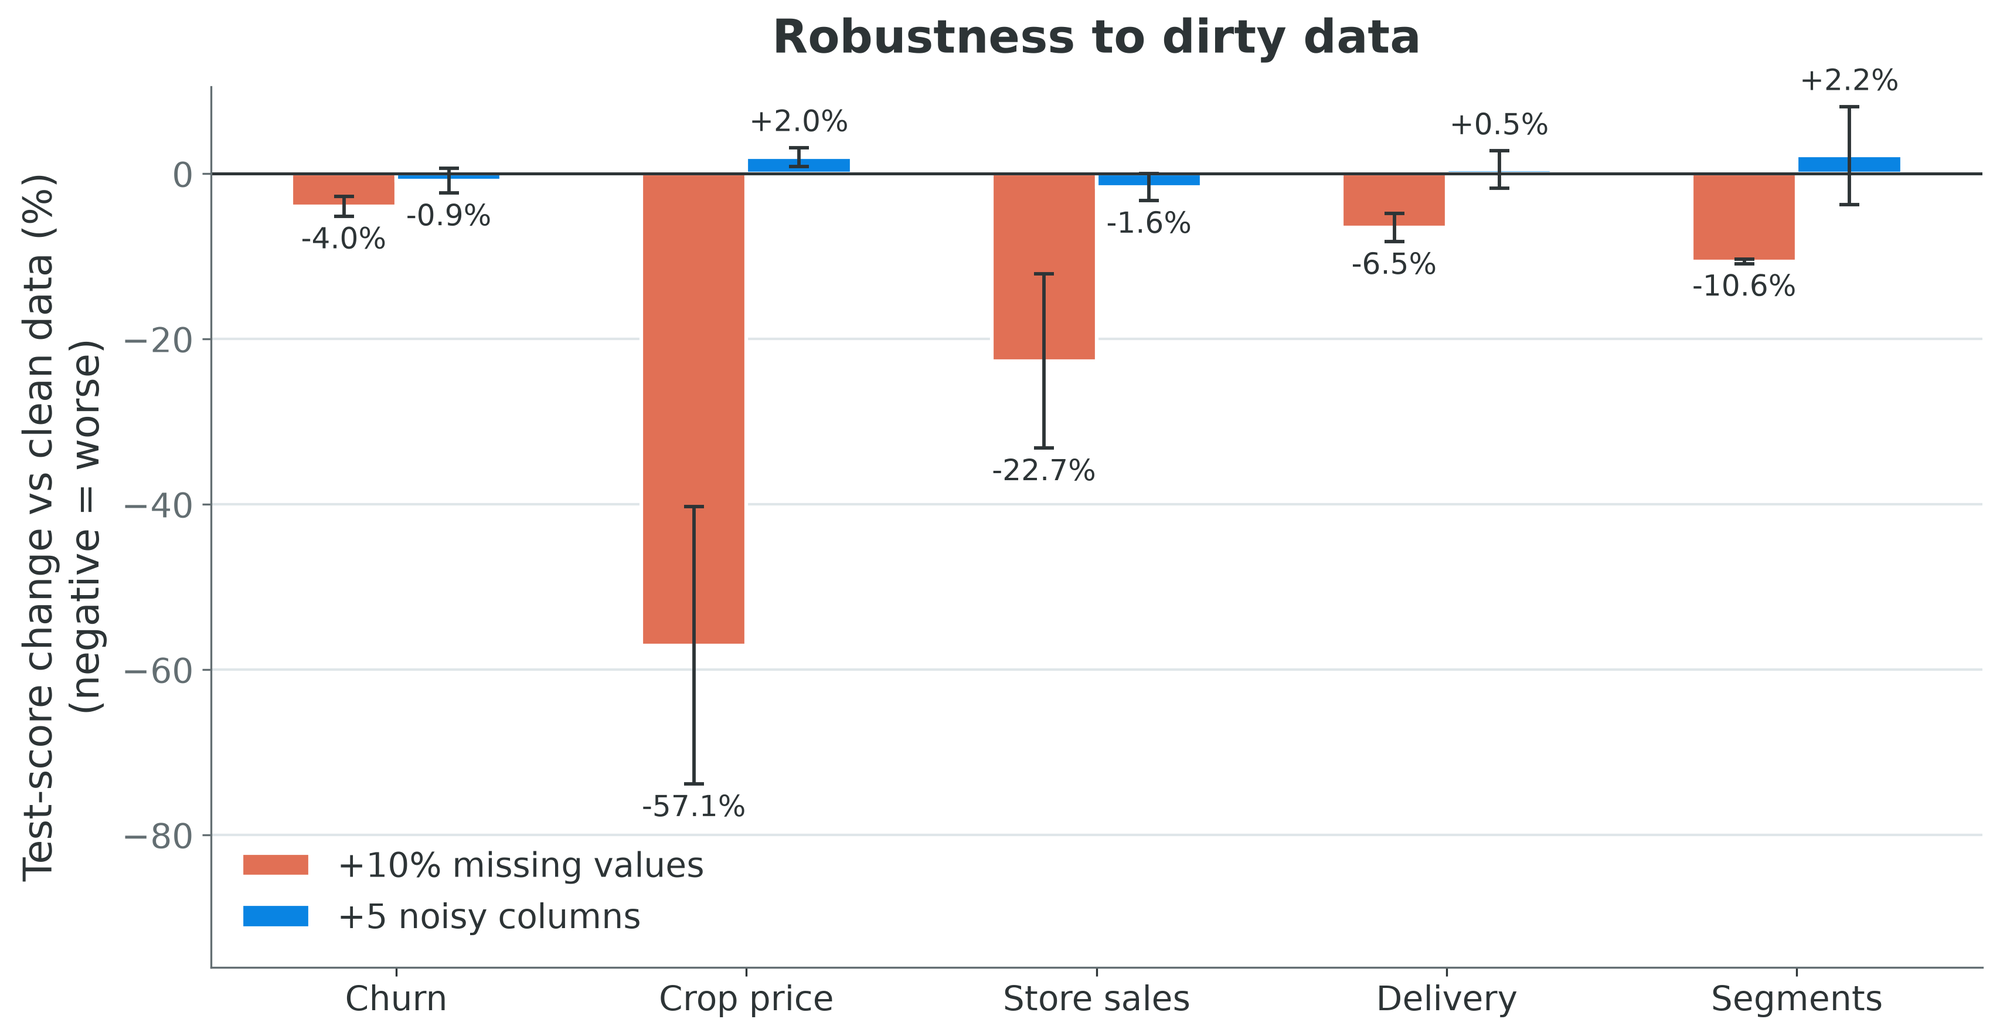
\includegraphics[width=\linewidth,height=7.3in,keepaspectratio]{figures/robustness.png}
  \caption{Robustness: change of the test score with 10\% extra missing values and with 5 noisy columns}\label{fig:7.4}
\end{figure}

Noise columns changed every score by at most 2.2\%: irrelevant features did not mislead the models. Missing values hurt more: 6 of the 10 perturbed settings stayed within 5\% of the clean score, and the largest losses were crop price (RMSE +57.1\%) and store sales (+22.7\%), plausibly because the simple imputation cannot recover the blanked information. Verification still passed in 29 of the 30 perturbed runs.

\FloatBarrier
\section{Impact of Threshold Tuning on Churn}\label{sec:7.6}

Churners are the minority (32.8\%), so a 0.5 cut-off is conservative and misses many of them. Over the three seeds, threshold tuning raises churn F1 from 0.561 \ensuremath{\pm}~0.006 (cut-off 0.5) to 0.649 \ensuremath{\pm}~0.028, a change of \ensuremath{-}13.4\% when it is removed (Table~\ref{tab:7.4}). Table~\ref{tab:7.6} shows the effect in more detail for a single demo run (seed 42): the selected logistic regression on the seed-42 split (Step 5 benchmark).

\begin{table}[H]
\centering
\linespread{1}\small
\setlength{\tabcolsep}{4pt}
\caption{Threshold tuning on churn (single demo run, seed 42: logistic regression, test split)}\label{tab:7.6}
\begin{tabular}{|>{\raggedright\arraybackslash\hspace{0pt}}p{\dimexpr 0.4386\linewidth-2\tabcolsep-2\arrayrulewidth\relax}|>{\raggedleft\arraybackslash\hspace{0pt}}p{\dimexpr 0.2225\linewidth-2\tabcolsep-2\arrayrulewidth\relax}|>{\raggedleft\arraybackslash\hspace{0pt}}p{\dimexpr 0.3389\linewidth-2\tabcolsep-2\arrayrulewidth\relax}|}
\hline
\rowcolor{tableheader}\textbf{Metric} & \textbf{Cut-off 0.5} & \textbf{Tuned cut-off 0.32} \\
\hline
F1 & 0.5579 & 0.6230 \\ \hline
Precision & 0.5824 & 0.5241 \\ \hline
Recall & 0.5354 & 0.7677 \\ \hline
Accuracy & 0.7200 & 0.6933 \\ \hline
ROC AUC (threshold-free) & 0.7738 & 0.7738 \\ \hline
\end{tabular}
\end{table}

The tuned cut-off \textbf{trades a little precision and accuracy for much higher recall}: in this run about 77\% of churners are found instead of 54\%, usually the right trade-off for a retention campaign. Over the three seeds the tuned thresholds were 0.32, 0.36 and 0.23.

The cut-off also drives the \textbf{risk tiers} (Figure~\ref{fig:5.5}; the same single demo run, seed 42, scored on all 3,000 customers). High risk starts at a probability of 0.4609 --- the larger of the threshold 0.32 and the 70th percentile --- and holds 900 customers (30.0\%); Medium (0.32 to 0.4609) holds 447 (14.9\%) and Low 1,653 (55.1\%). The strongest drivers were \code{contract\_\allowbreak{}type} (34\% of the explanation), \code{tenure\_\allowbreak{}months} (20\%) and \code{payment\_\allowbreak{}method} (13\%). Moving the high-risk customers to a two-year contract would lower their average predicted churn probability from 0.651 to 0.193 according to the model --- a statement about the model, not a guaranteed effect of a campaign.

\FloatBarrier
\section{Clustering: Adjusted Rand Index versus Rand Index}\label{sec:7.7}

AutoML-Agent scores clustering with the Rand index (RI) \cite{ref17}, the share of record pairs on which clustering and ground truth agree. Because most pairs belong to different groups, RI rewards over-splitting and is not corrected for chance: a random assignment into four groups already scores about 0.62 here, and in a first run an untuned k-means with 8 clusters beat the tuned 4-cluster model on RI. The \textbf{adjusted Rand index} \cite{ref18}, ARI = (RI \ensuremath{-} E[RI]) / (max(RI) \ensuremath{-} E[RI]), scores about 0 for random labels and 1 for a perfect match. IDSS therefore uses ARI wherever ground truth exists and still reports RI (Table~\ref{tab:7.7}).

The investigation also exposed a bug: the Gaussian mixture ran a single EM initialisation and, for some seeds, its refit stopped in a poor optimum (ARI \ensuremath{\approx} 0.53 instead of 0.84), which made added noise look like an improvement. It now uses several initialisations (5, or 3 above 20,000 rows). Segments was re-run after both changes; the replaced runs are kept under \code{superseded} in \code{evaluation.json}.

\begin{table}[H]
\centering
\linespread{1}\small
\setlength{\tabcolsep}{4pt}
\caption{Clustering results with ARI and RI (Segments, mean \ensuremath{\pm}~std over 3 seeds)}\label{tab:7.7}
\begin{tabular}{|>{\raggedright\arraybackslash\hspace{0pt}}p{\dimexpr 0.3248\linewidth-2\tabcolsep-2\arrayrulewidth\relax}|>{\raggedright\arraybackslash\hspace{0pt}}p{\dimexpr 0.3656\linewidth-2\tabcolsep-2\arrayrulewidth\relax}|>{\raggedleft\arraybackslash\hspace{0pt}}p{\dimexpr 0.1548\linewidth-2\tabcolsep-2\arrayrulewidth\relax}|>{\raggedleft\arraybackslash\hspace{0pt}}p{\dimexpr 0.1548\linewidth-2\tabcolsep-2\arrayrulewidth\relax}|}
\hline
\rowcolor{tableheader}\textbf{Configuration} & \textbf{Models chosen} & \textbf{ARI \ensuremath{\uparrow}} & \textbf{RI \ensuremath{\uparrow}} \\
\hline
Full system & Gaussian mixture \ensuremath{\times} 3 & 0.816 \ensuremath{\pm}~0.045 & 0.930 \ensuremath{\pm}~0.017 \\ \hline
\ensuremath{-} hyperparameter tuning & agglomerative \ensuremath{\times} 2, k-means & 0.523 \ensuremath{\pm}~0.078 & 0.804 \ensuremath{\pm}~0.046 \\ \hline
Single-model baseline & k-means \ensuremath{\times} 3 & 0.508 \ensuremath{\pm}~0.012 & 0.841 \ensuremath{\pm}~0.006 \\ \hline
Full system, +10\% missing & agglomerative, Gaussian mixture \ensuremath{\times} 2 & 0.729 \ensuremath{\pm}~0.042 & 0.896 \ensuremath{\pm}~0.014 \\ \hline
Full system, +5 noisy columns & Gaussian mixture \ensuremath{\times} 3 & 0.833 \ensuremath{\pm}~0.053 & 0.936 \ensuremath{\pm}~0.019 \\ \hline
\end{tabular}
\end{table}

The random baseline scored RI = 0.625 but ARI = 0.004, which shows why the chance-corrected index is fairer.

\FloatBarrier
\section{Efficiency}\label{sec:7.8}

With the fast budget the search plus refit took 2.7 s (Segments) to 19.8 s (Churn) on average; Delivery averaged 72.2 s with a wide spread because one seed triggered a full-budget re-plan (157.9 s). Inference took 0.016 to 0.201 ms per row, preprocessing included; the time-series pipeline is the slowest per row, probably because it builds lag and rolling features at prediction time (Figure~\ref{fig:7.5}).

\begin{figure}[htbp]
  \centering
  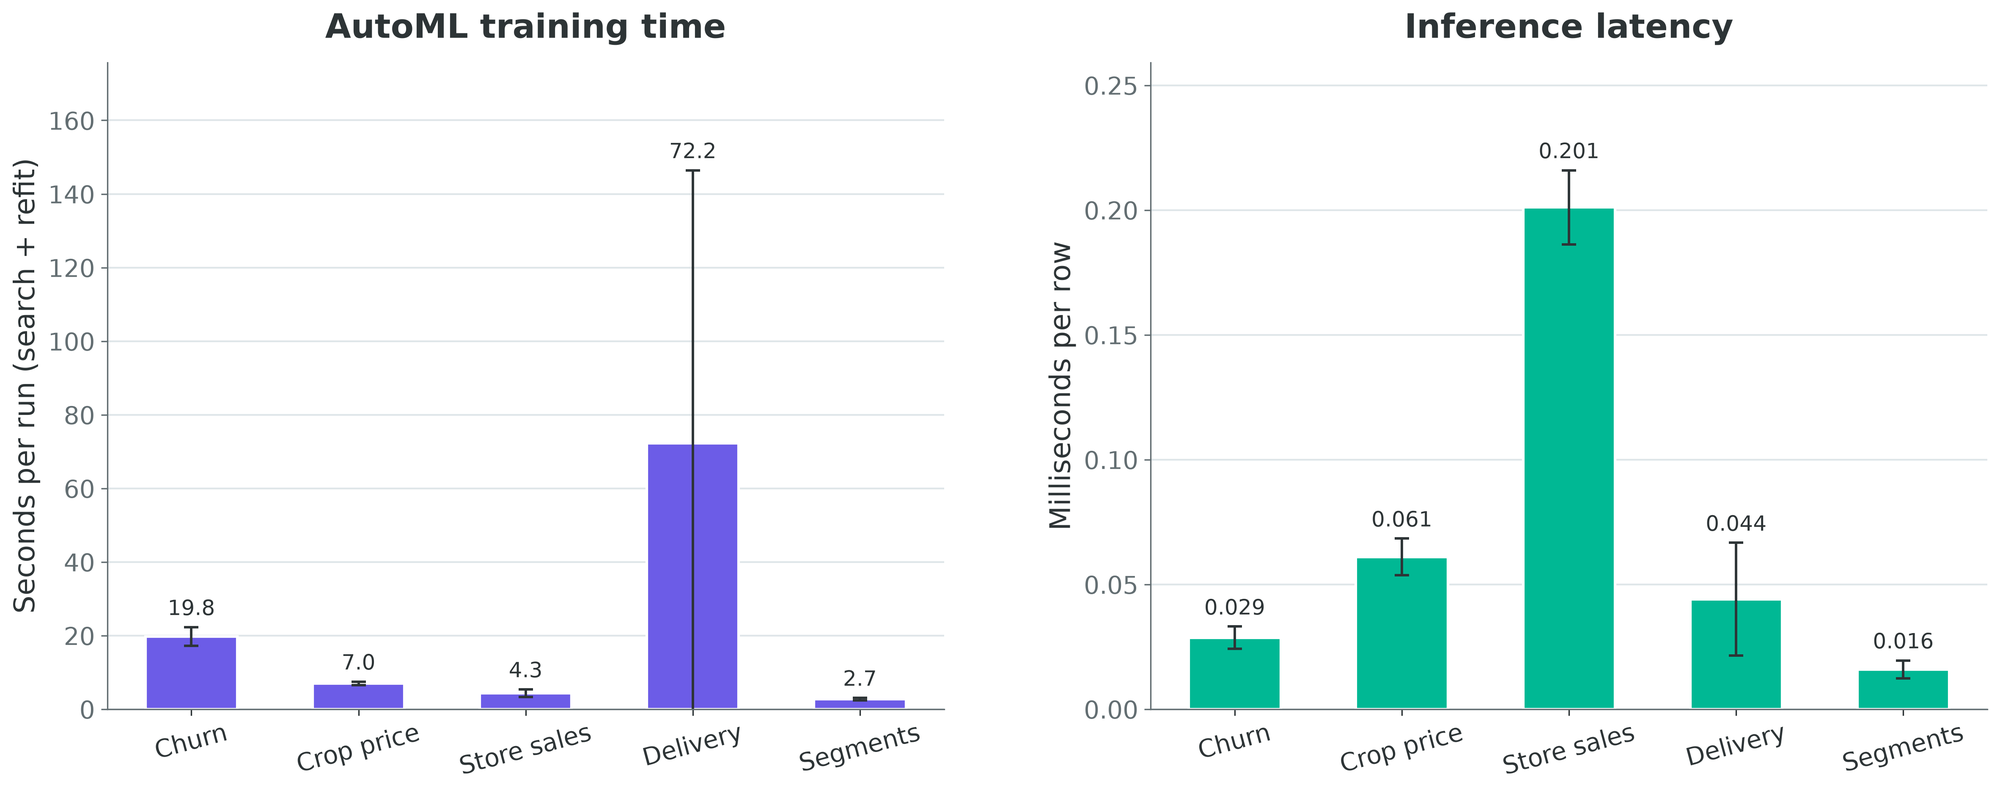
\includegraphics[width=\linewidth,height=7.3in,keepaspectratio]{figures/efficiency.png}
  \caption{Efficiency: AutoML training time per run and inference latency per row}\label{fig:7.5}
\end{figure}

\FloatBarrier
\section{Verification Outcomes}\label{sec:7.9}

Verification passed in 14 of 15 clean full-system runs. Table~\ref{tab:7.8} lists the full-system and variant runs that did not pass; all failed the overfitting check (train--test gap \ensuremath{\geq} 0.15 on the primary 0--1 metric).

\begin{table}[H]
\centering
\linespread{1}\footnotesize
\setlength{\tabcolsep}{4pt}
\caption{Runs that did not pass verification}\label{tab:7.8}
\begin{tabular}{|>{\raggedright\arraybackslash\hspace{0pt}}p{\dimexpr 0.1315\linewidth-2\tabcolsep-2\arrayrulewidth\relax}|>{\raggedleft\arraybackslash\hspace{0pt}}p{\dimexpr 0.0820\linewidth-2\tabcolsep-2\arrayrulewidth\relax}|>{\raggedright\arraybackslash\hspace{0pt}}p{\dimexpr 0.2114\linewidth-2\tabcolsep-2\arrayrulewidth\relax}|>{\raggedright\arraybackslash\hspace{0pt}}p{\dimexpr 0.1405\linewidth-2\tabcolsep-2\arrayrulewidth\relax}|>{\raggedleft\arraybackslash\hspace{0pt}}p{\dimexpr 0.0974\linewidth-2\tabcolsep-2\arrayrulewidth\relax}|>{\raggedright\arraybackslash\hspace{0pt}}p{\dimexpr 0.1563\linewidth-2\tabcolsep-2\arrayrulewidth\relax}|>{\raggedright\arraybackslash\hspace{0pt}}p{\dimexpr 0.1809\linewidth-2\tabcolsep-2\arrayrulewidth\relax}|}
\hline
\rowcolor{tableheader}\textbf{Dataset} & \textbf{Seed} & \textbf{Configuration} & \textbf{Selected model} & \textbf{Test F1} & \textbf{Re-planned} & \textbf{Outcome} \\
\hline
Delivery & 44 & Full system, clean & LightGBM & 0.636 & Yes & Still failing; DONE, flagged \textit{not verified} \\ \hline
Delivery & 42 & Full system, +10\% missing & XGBoost & 0.625 & Yes & Still failing; flagged \textit{not verified} \\ \hline
Churn & 43 & \ensuremath{-} threshold tuning & LightGBM & 0.568 & Yes & Still failing; flagged \textit{not verified} \\ \hline
\end{tabular}
\end{table}

The single default LightGBM failed the same check in 9 of 15 runs (Churn, Store sales and Delivery on every seed). These cases show the verifier working as intended: when a boosted-tree model fitted the training rows much better than the test rows and the full-budget re-plan could not fix it, the system completed the analysis but labelled the result \textit{not verified} instead of presenting an over-fitted model as trustworthy.

\FloatBarrier
\section{Discussion}\label{sec:7.10}

\textbf{Strengths.}

\begin{itemize}
  \item \textbf{Every run finishes} (SR = 1.00) because the LLM plans but never writes training code.
  \item \textbf{Better than trivial on every dataset}, with RMSE reductions of 85.1\% and 60.5\% and an ARI of 0.816 against about 0.
  \item \textbf{Each component contributes}: search, tuning and threshold tuning raise CS from 0.854 to 0.900, and threshold tuning alone raises F1 on the imbalanced churn data from 0.561 to 0.649 (\ensuremath{-}13.4\% without it).
  \item \textbf{Robust to irrelevant features}: five noise columns changed scores by at most 2.2\%.
  \item \textbf{Honest self-assessment}: the test split was read once in every run, baselines used the same split, over-fitting was reported rather than hidden, and the evaluation itself caught a misleading metric and an engine bug.
  \item \textbf{Decisions, not only scores}: risk tiers with stated cut-offs, drivers and actions with expected effects, and a brief whose numbers are grounded in computed facts.
\end{itemize}

\textbf{Limitations.}

\begin{itemize}
  \item \textbf{Synthetic data}: real business data is noisier and may contain drift, label noise or leakage, so these results are not performance on real data.
  \item \textbf{The LLM path is not benchmarked}: the evaluation ran offline, so parsing, the knowledge brief, the LLM review and the written insights used their fallbacks; the results measure the engine and the pipeline.
  \item \textbf{Small study}: three seeds, the fast budget and one machine.
  \item \textbf{Missing values} are the main weakness (crop price RMSE +57.1\%), and on Delivery the single re-plan did not cure over-fitting; a different strategy on the second attempt would be needed.
  \item \textbf{Correlation, not causation}: drivers, what-if results and counterfactual actions describe the model's response, not real-world effects, which only an experiment can measure.
\end{itemize}

\FloatBarrier
\section{Summary}\label{sec:7.11}

On five synthetic, seeded datasets IDSS completed every run (SR = 1.00) with NPS = 0.800 and CS = 0.900, beat the baseline everywhere and passed verification in 14 of 15 full-system runs. The ablation showed the value of model search, tuning and especially threshold tuning; the robustness study showed that noise is harmless while missing values hurt; ARI made the clustering evaluation fair; and the verifier flagged over-fitted runs instead of hiding them.
